\subsection{Spezielle Punkte und Eigenschaften von Kurven}
\label{speziellePte}
\subsubsection{Extrema und Wendepunkte bestimmen}
\begin{LA}
    {Zuordnung von Graphenausschnitten}{zuordnungGraphen}
    In den Koordinatensystemen oben sind Ausschnitte von sechs Funktionsgraphen gezeichnet. In den Koordinatensystemen unten Ausschnitte von sechs Ableitungen. Welcher Ableitung passt zu welchem Graph?


    \begin{center}
        
    
    \begin{tabular}{|c|c|c|}
        \hline
        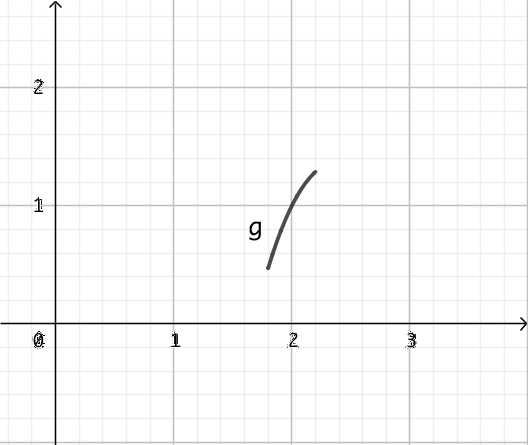
\includegraphics[width = 4cm]{media/Graph und Ableitung Kopie/Graph 1.png} &
        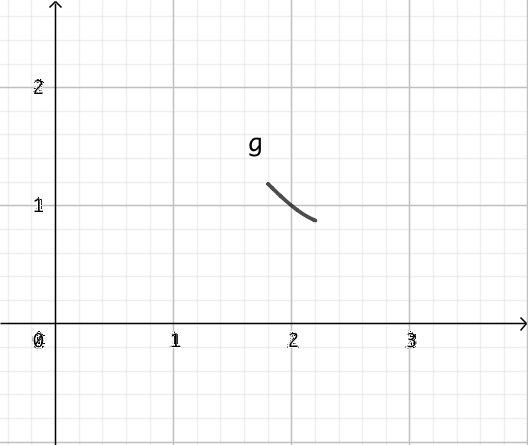
\includegraphics[width = 4cm]{media/Graph und Ableitung Kopie/Graph2.png} &
        \includegraphics[width = 4cm]{media/Graph und Ableitung Kopie/Graph3.png} \\  \hline

        \includegraphics[width = 4cm]{media/Graph und Ableitung Kopie/Graph4.png} & 
        \includegraphics[width = 4cm]{media/Graph und Ableitung Kopie/Graph5.png} & 
        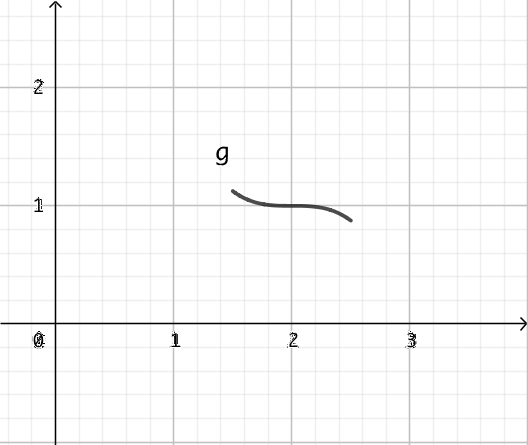
\includegraphics[width = 4cm]{media/Graph und Ableitung Kopie/graph6.png} \\ \hline
        \hline

        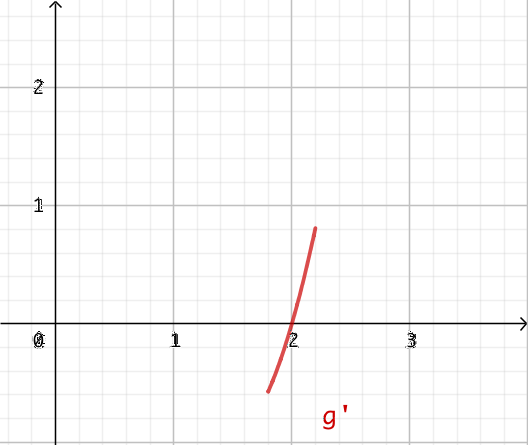
\includegraphics[width = 4cm]{media/Graph und Ableitung Kopie/ableitung 4.png} &
        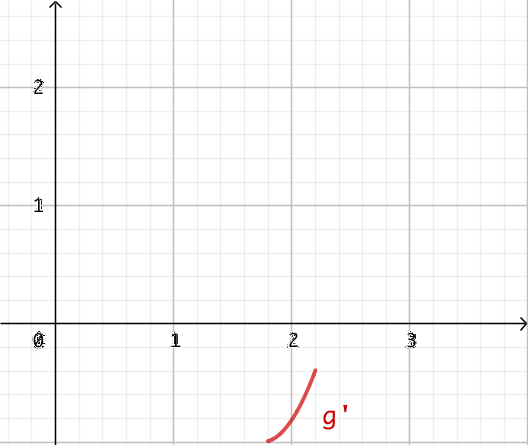
\includegraphics[width = 4cm]{media/Graph und Ableitung Kopie/Ableitung 2.png} &
        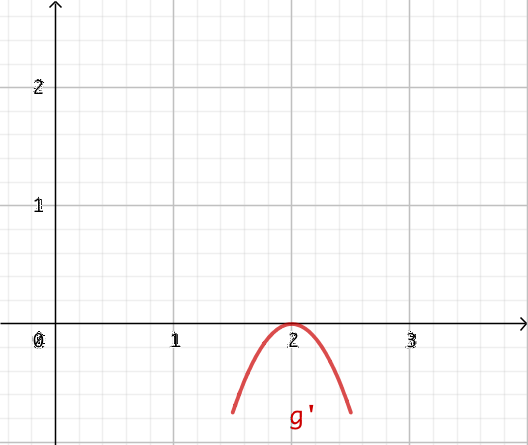
\includegraphics[width = 4cm]{media/Graph und Ableitung Kopie/ableitung6.png} \\ \hline

        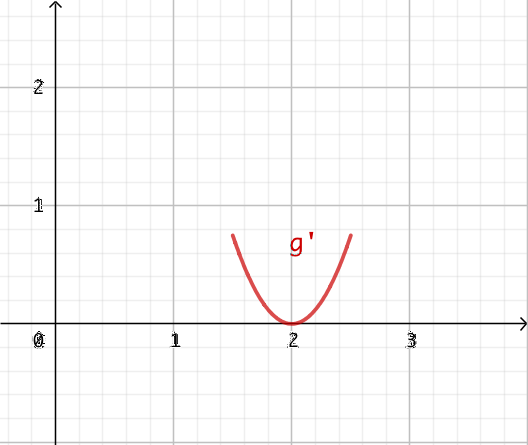
\includegraphics[width = 4cm]{media/Graph und Ableitung Kopie/ableitung5.png} & 
        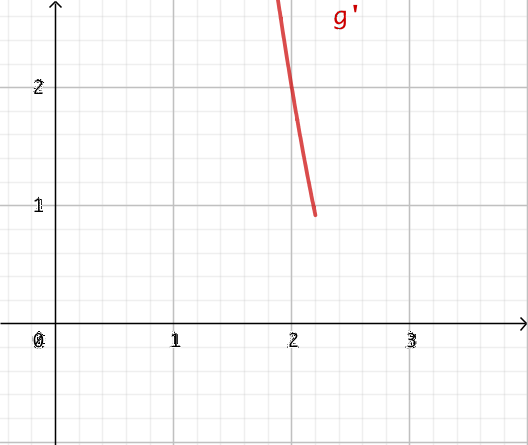
\includegraphics[width = 4cm]{media/Graph und Ableitung Kopie/ableitung 1.png} & 
        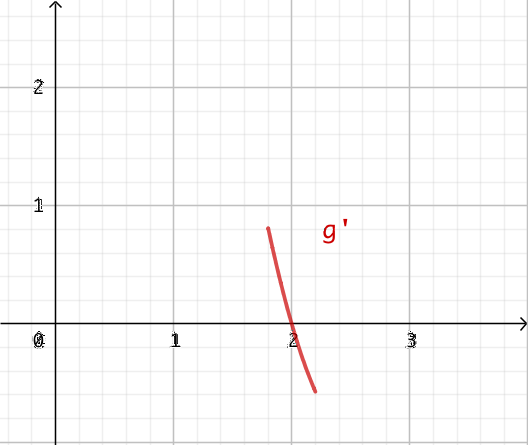
\includegraphics[width = 4cm]{media/Graph und Ableitung Kopie/ableitung3.png} \\ \hline
    \end{tabular}
\end{center}



\end{LA}
\clearpage

Aufgrund des Vorzeichens der ersten Ableitung einer Funktion kann man Rückschlüsse auf die Gestalt des ursprünglichen Graphen ziehen. Erste Erkenntnisse aus der Lernaufgabe \ref{LA:zuordnungGraphen} lassen sich wie folgt zusammenfassen:

Sei $f$ eine differenzierbare Funktion mit Definitionsbereich $\DD_f$. Sei $I \subset \DD_f$ ein Intervall und $x_0 \in \DD_f$. Dann gilt:

\begin{center}
    \begin{tabular}{| m{10cm} | m{4cm}|} \hline
        $f$ ist im Intervall $I$ \emph{monoton wachsend} $$\iff$$ $ f'(x)\ge 0$ für alle $x\in I$ & 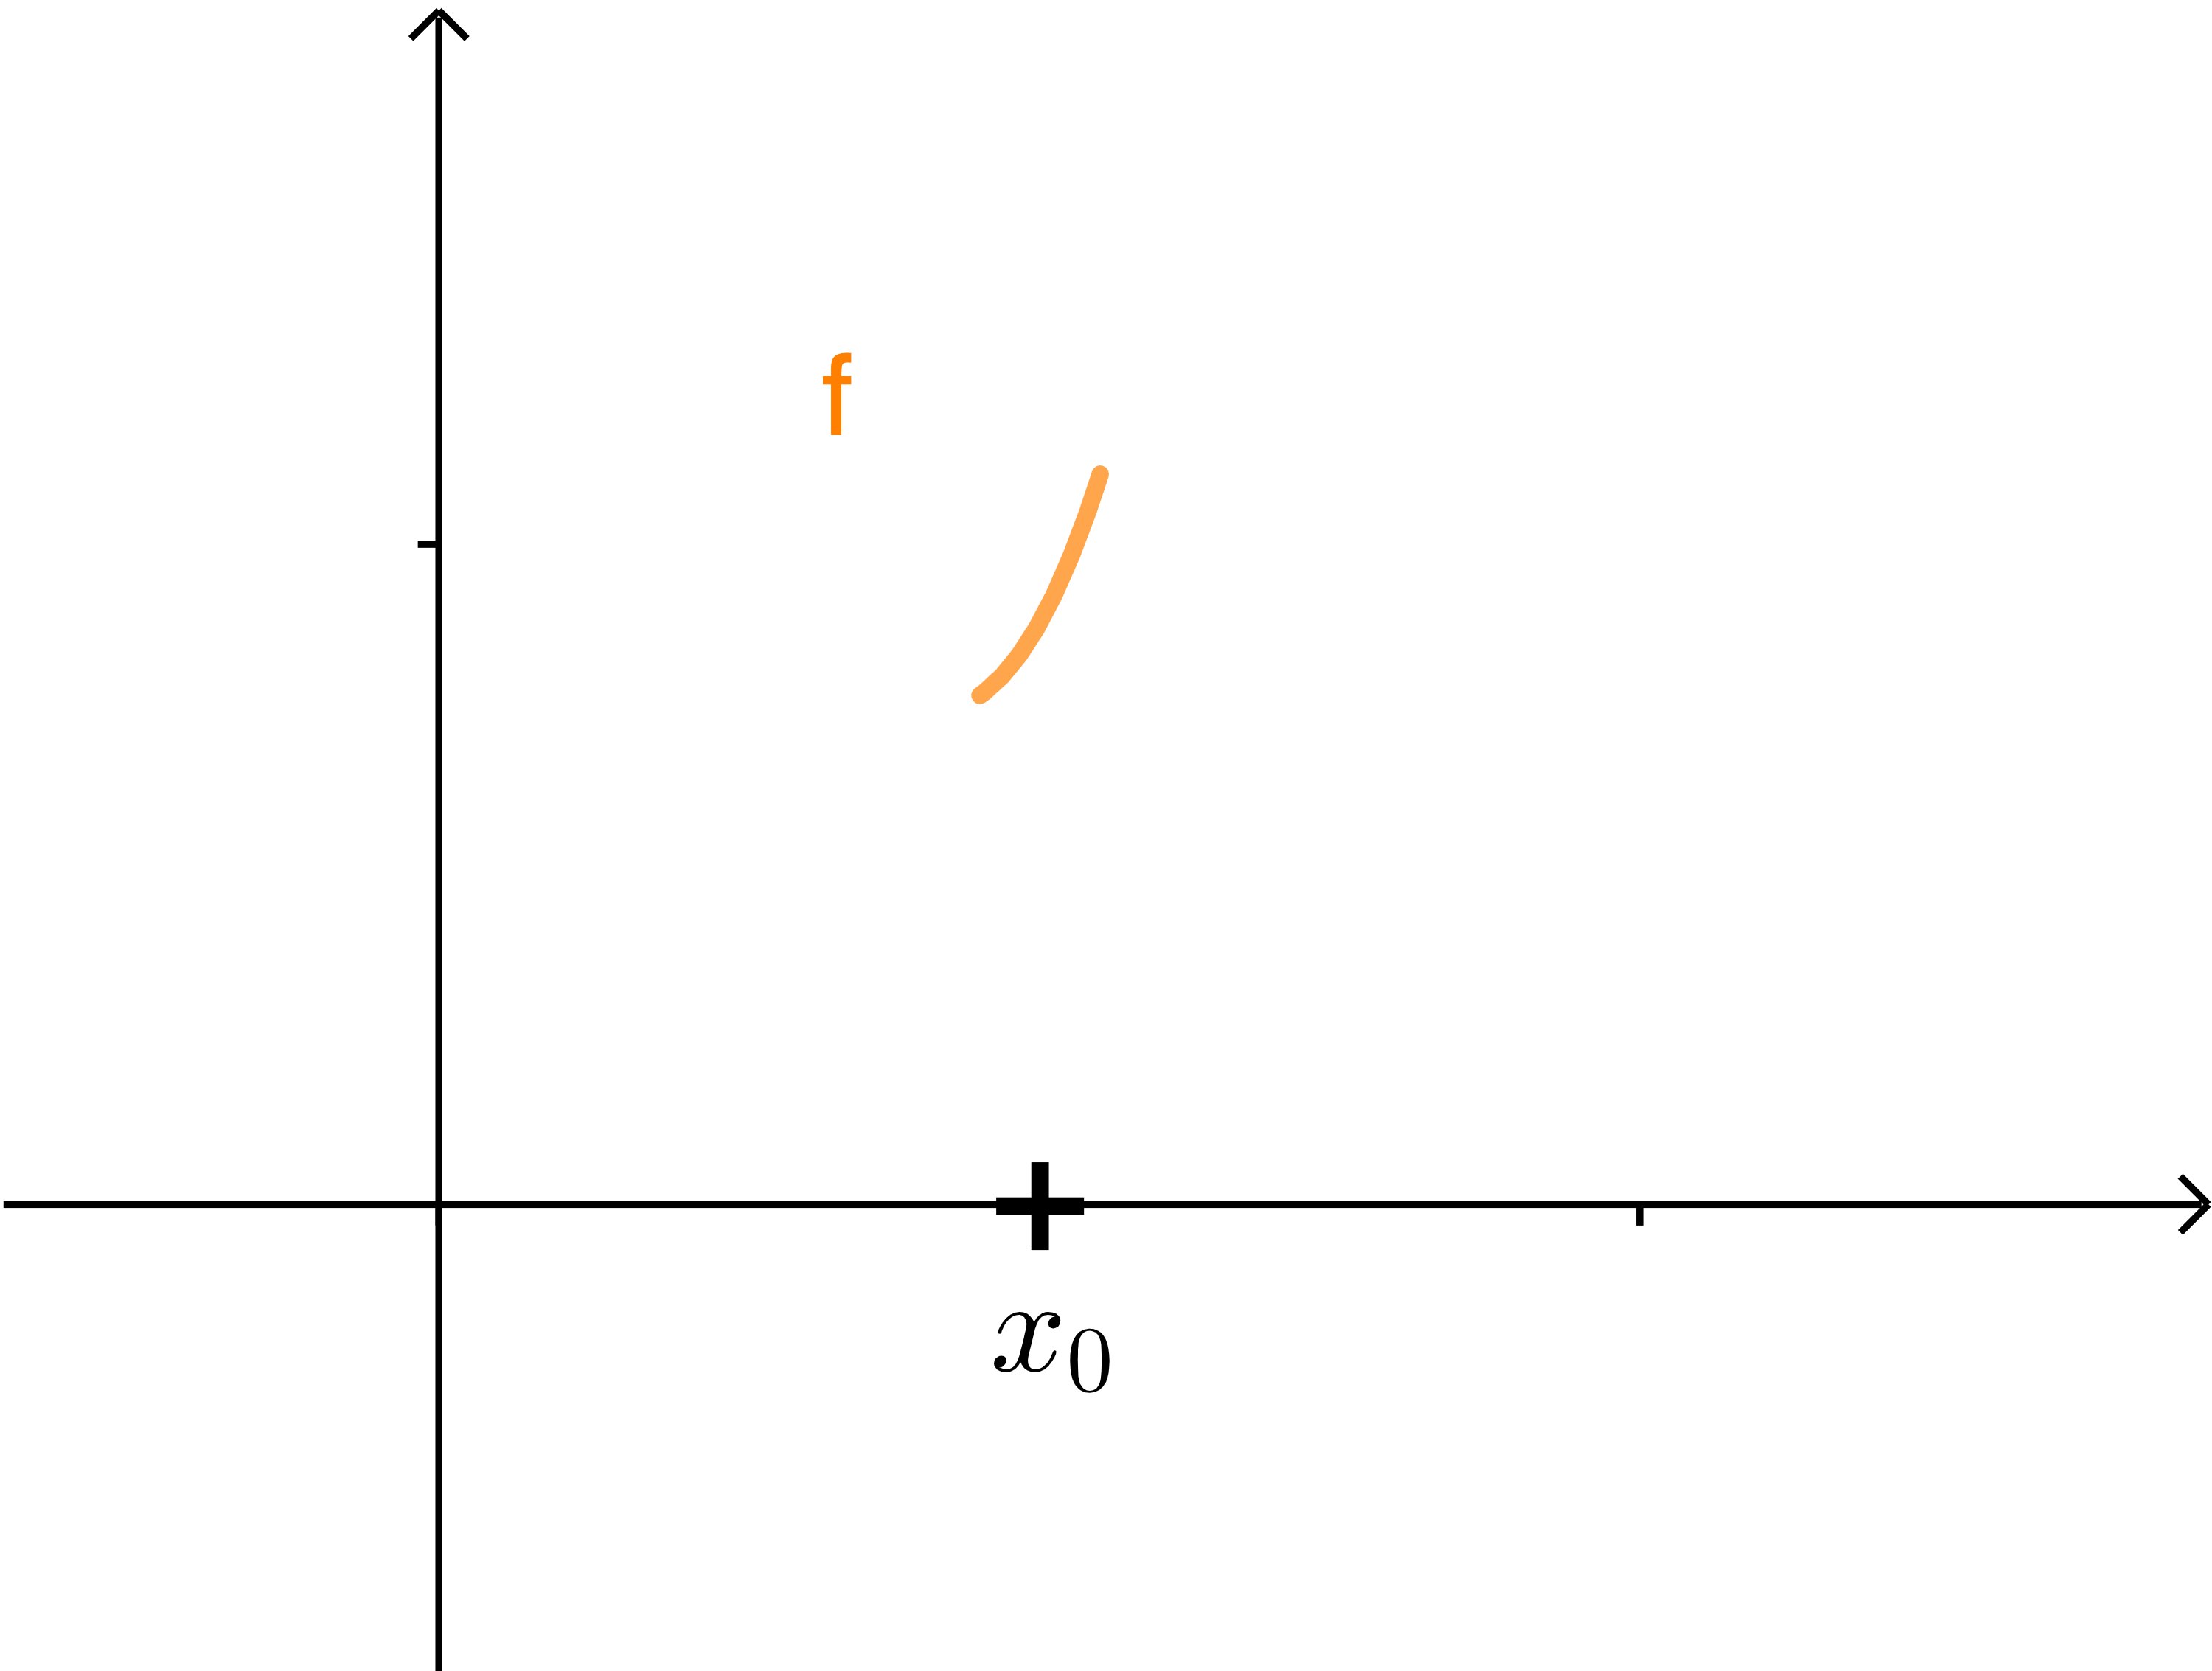
\includegraphics[width = 4cm]{media/Graph und Ableitung Kopie/wachsend.png}\\ \hline
        $f$ ist im Intervall $I$ \emph{monoton fallend} $$\iff$$  $f'(x) \le 0$ für alle $x\in I$ &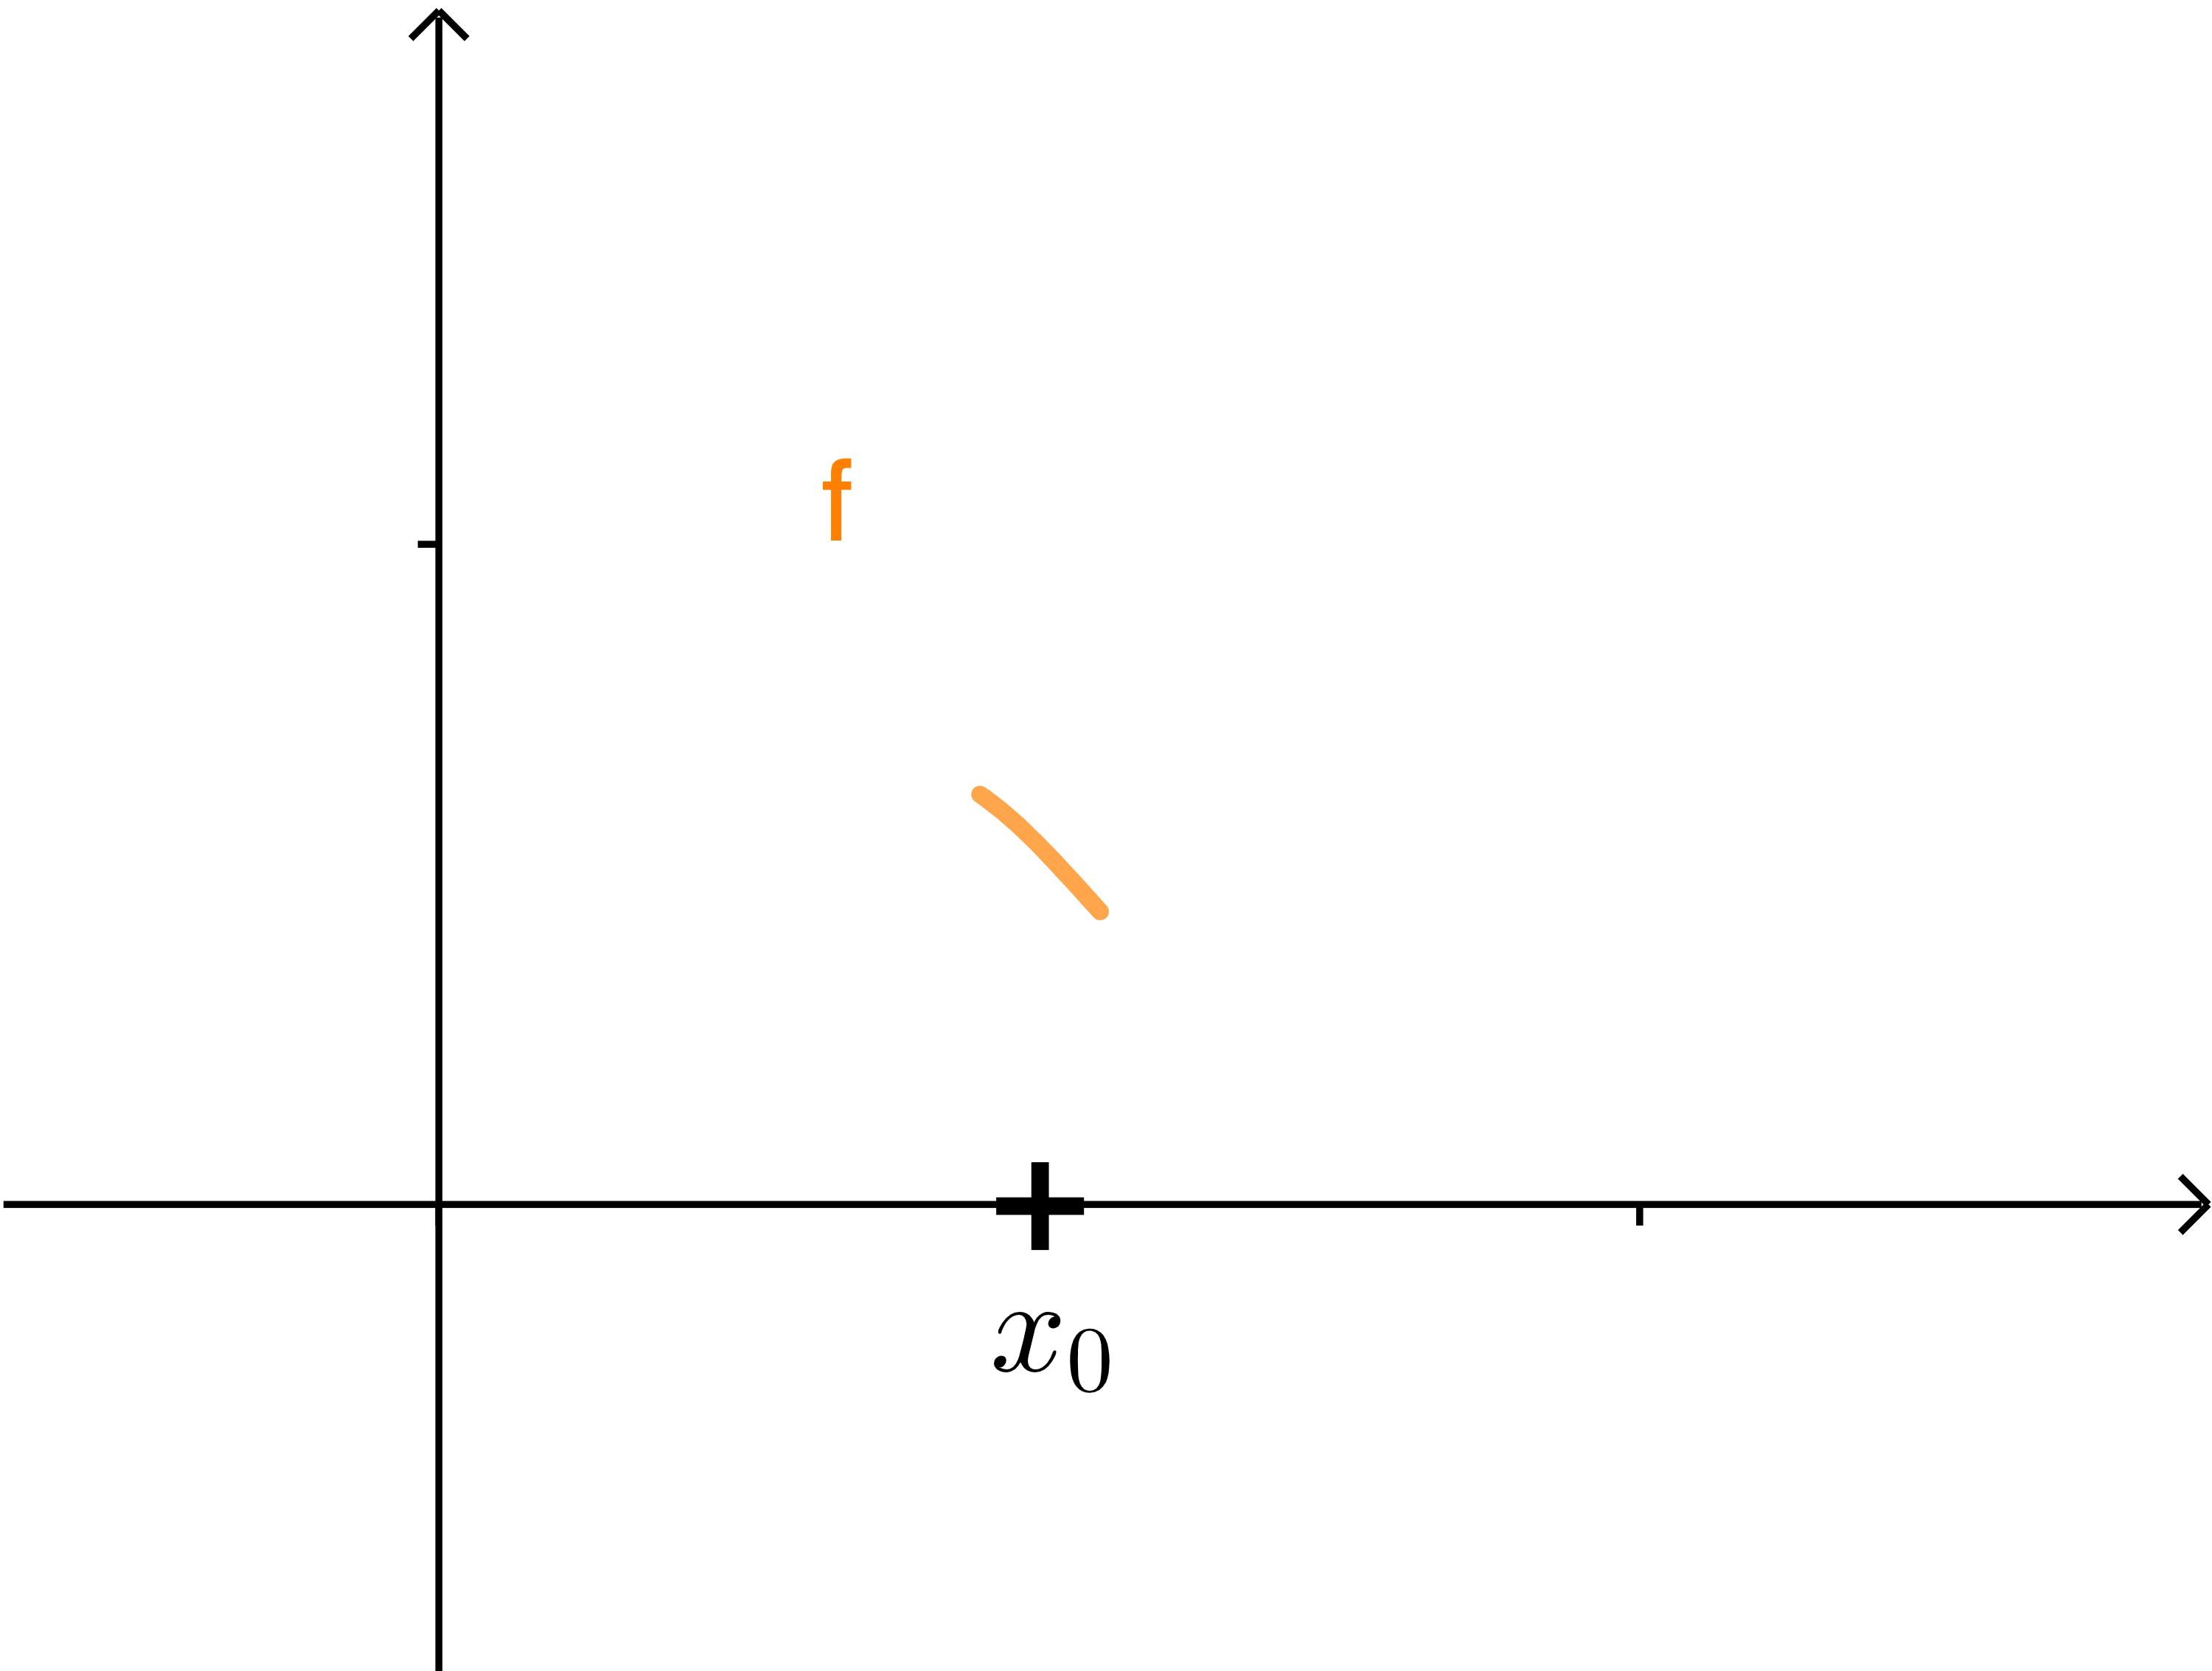
\includegraphics[width = 4cm]{media/Graph und Ableitung Kopie/fallend.png}\\ \hline
        $f$ hat an der Stelle $x_0$ ein \emph{lokales Maximum} (auch Hochpunkt genannt) $$\iff$$ $f'$ wechselt an der Stelle $x_0$ das Vorzeichen von positiv zu negativ. & 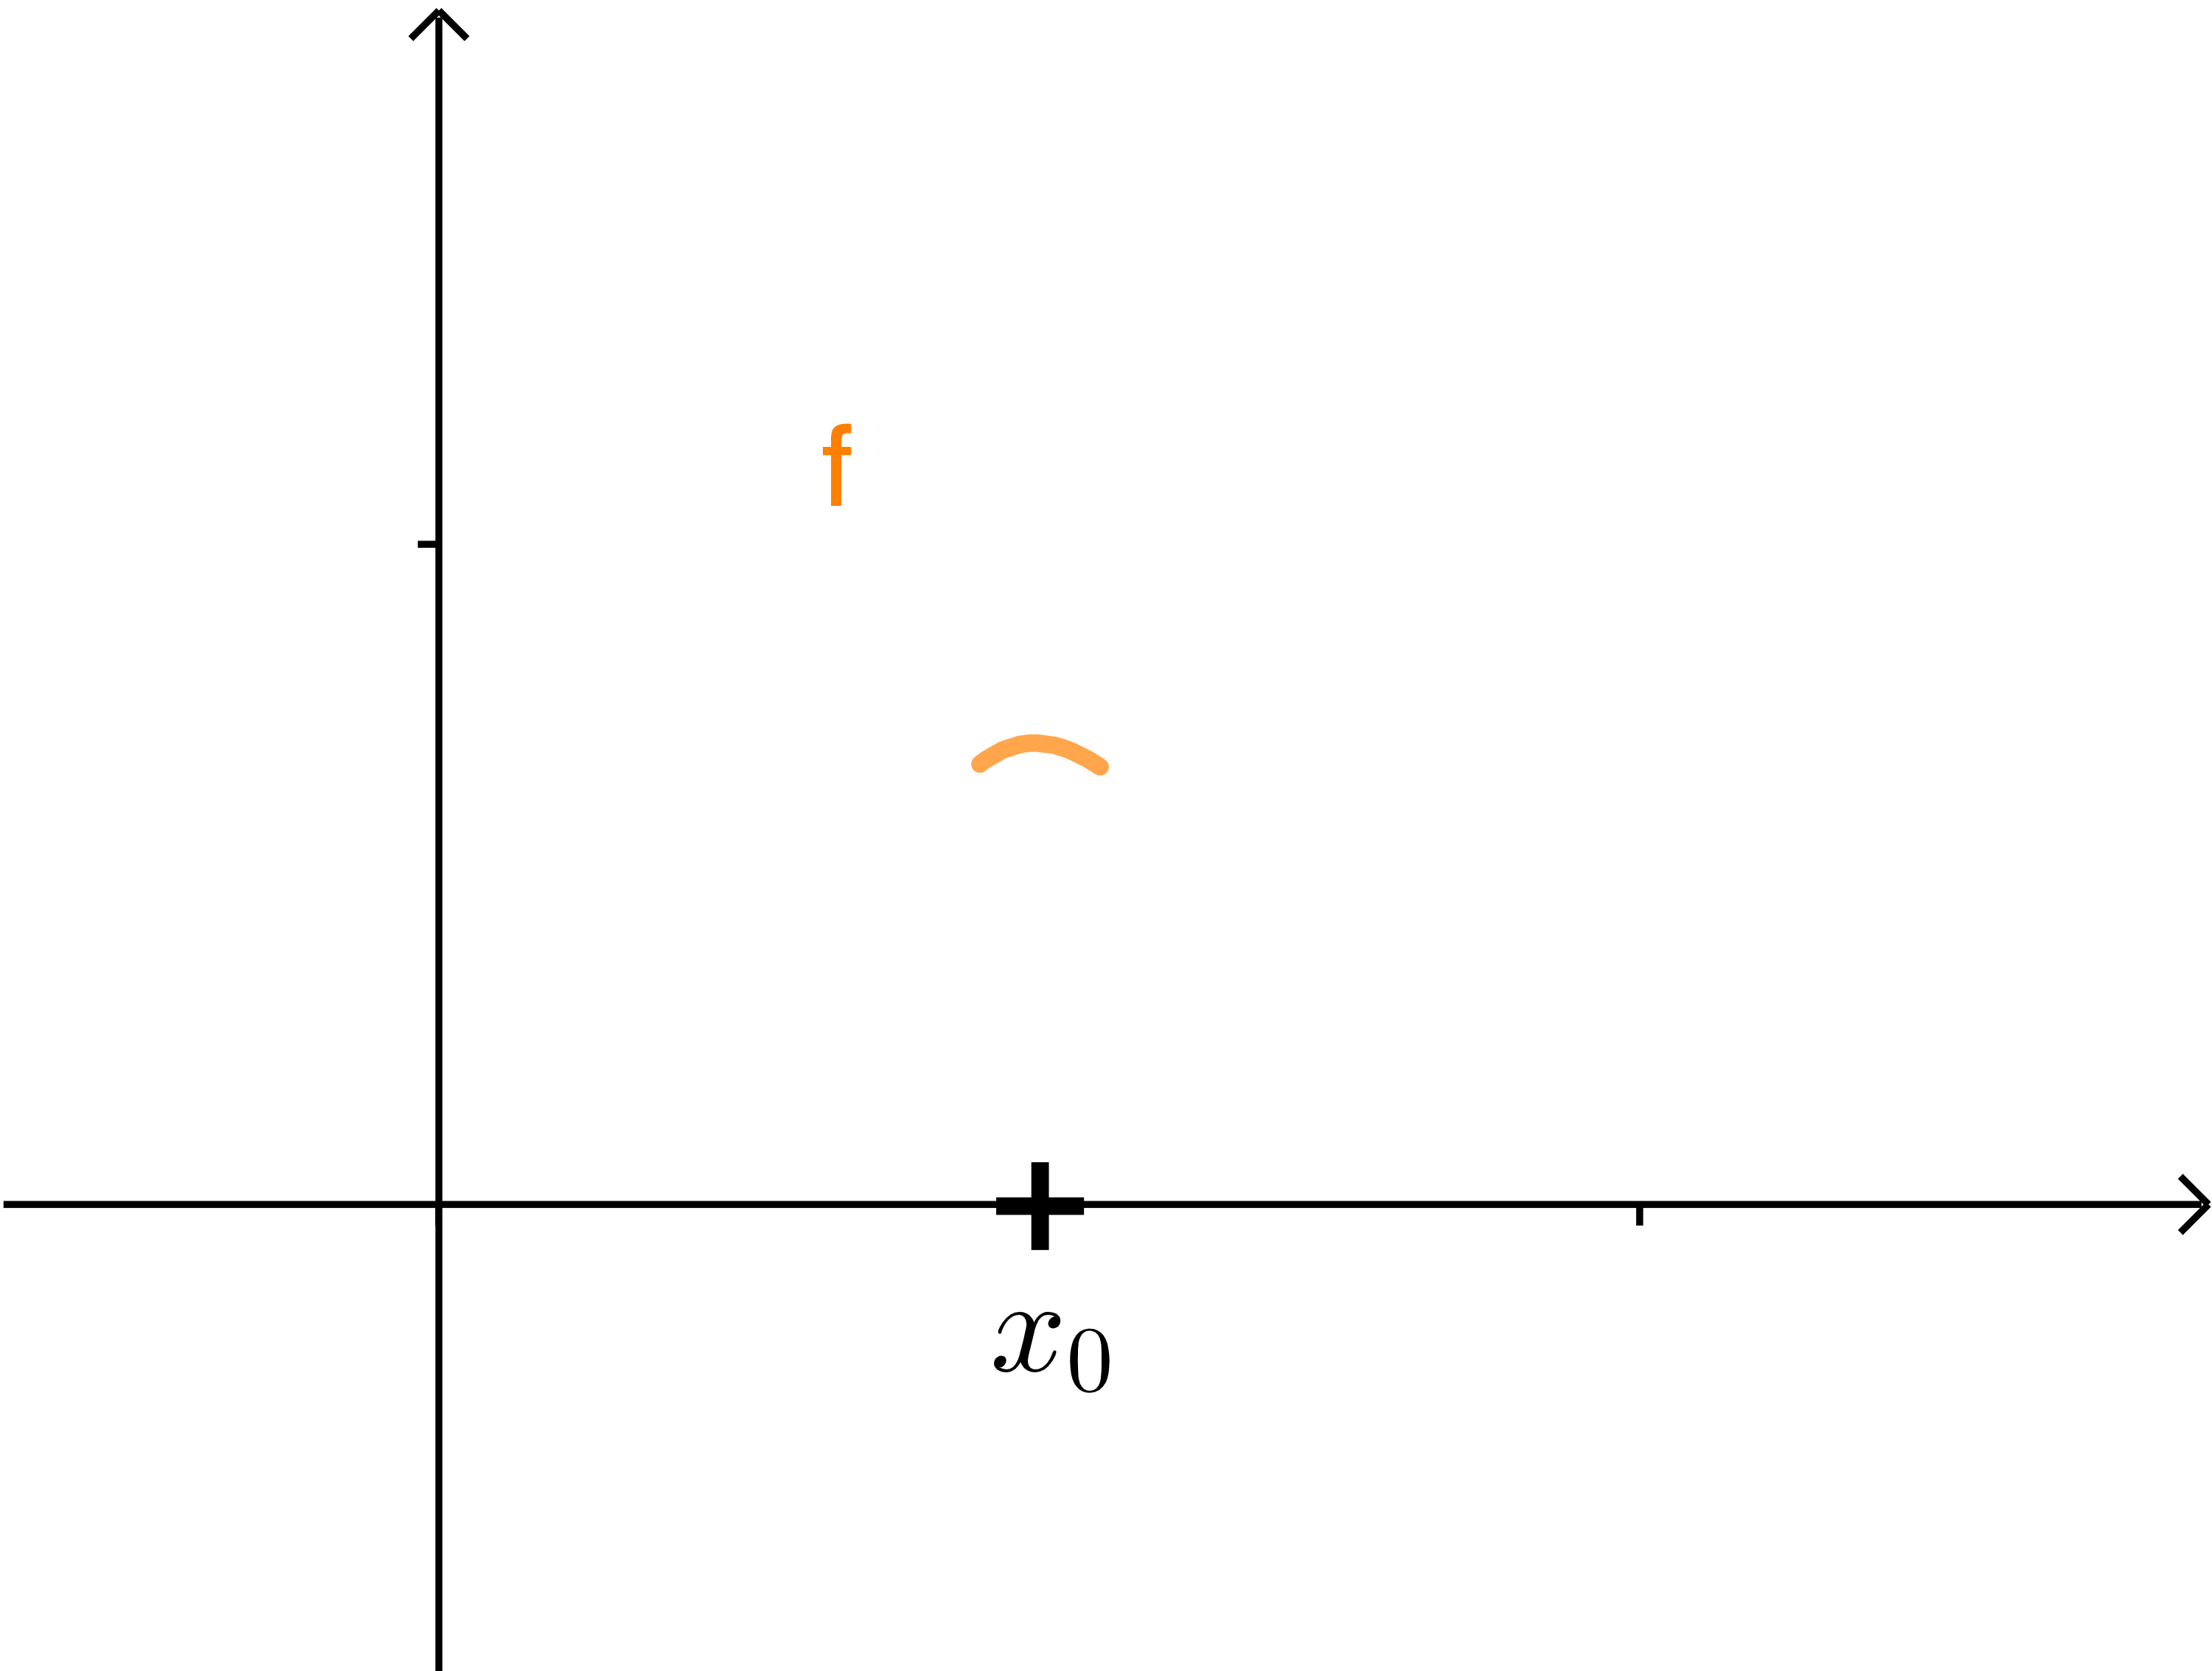
\includegraphics[width = 4cm]{media/Graph und Ableitung Kopie/maxx.png} \\ \hline
        $f$ hat an der Stelle $x_0$ ein \emph{lokales Minimum} (auch Tiefpunkt genannt) $$\iff$$  $f'$ wechselt an der Stelle $x_0$ das Vorzeichen von negativ zu positiv. & 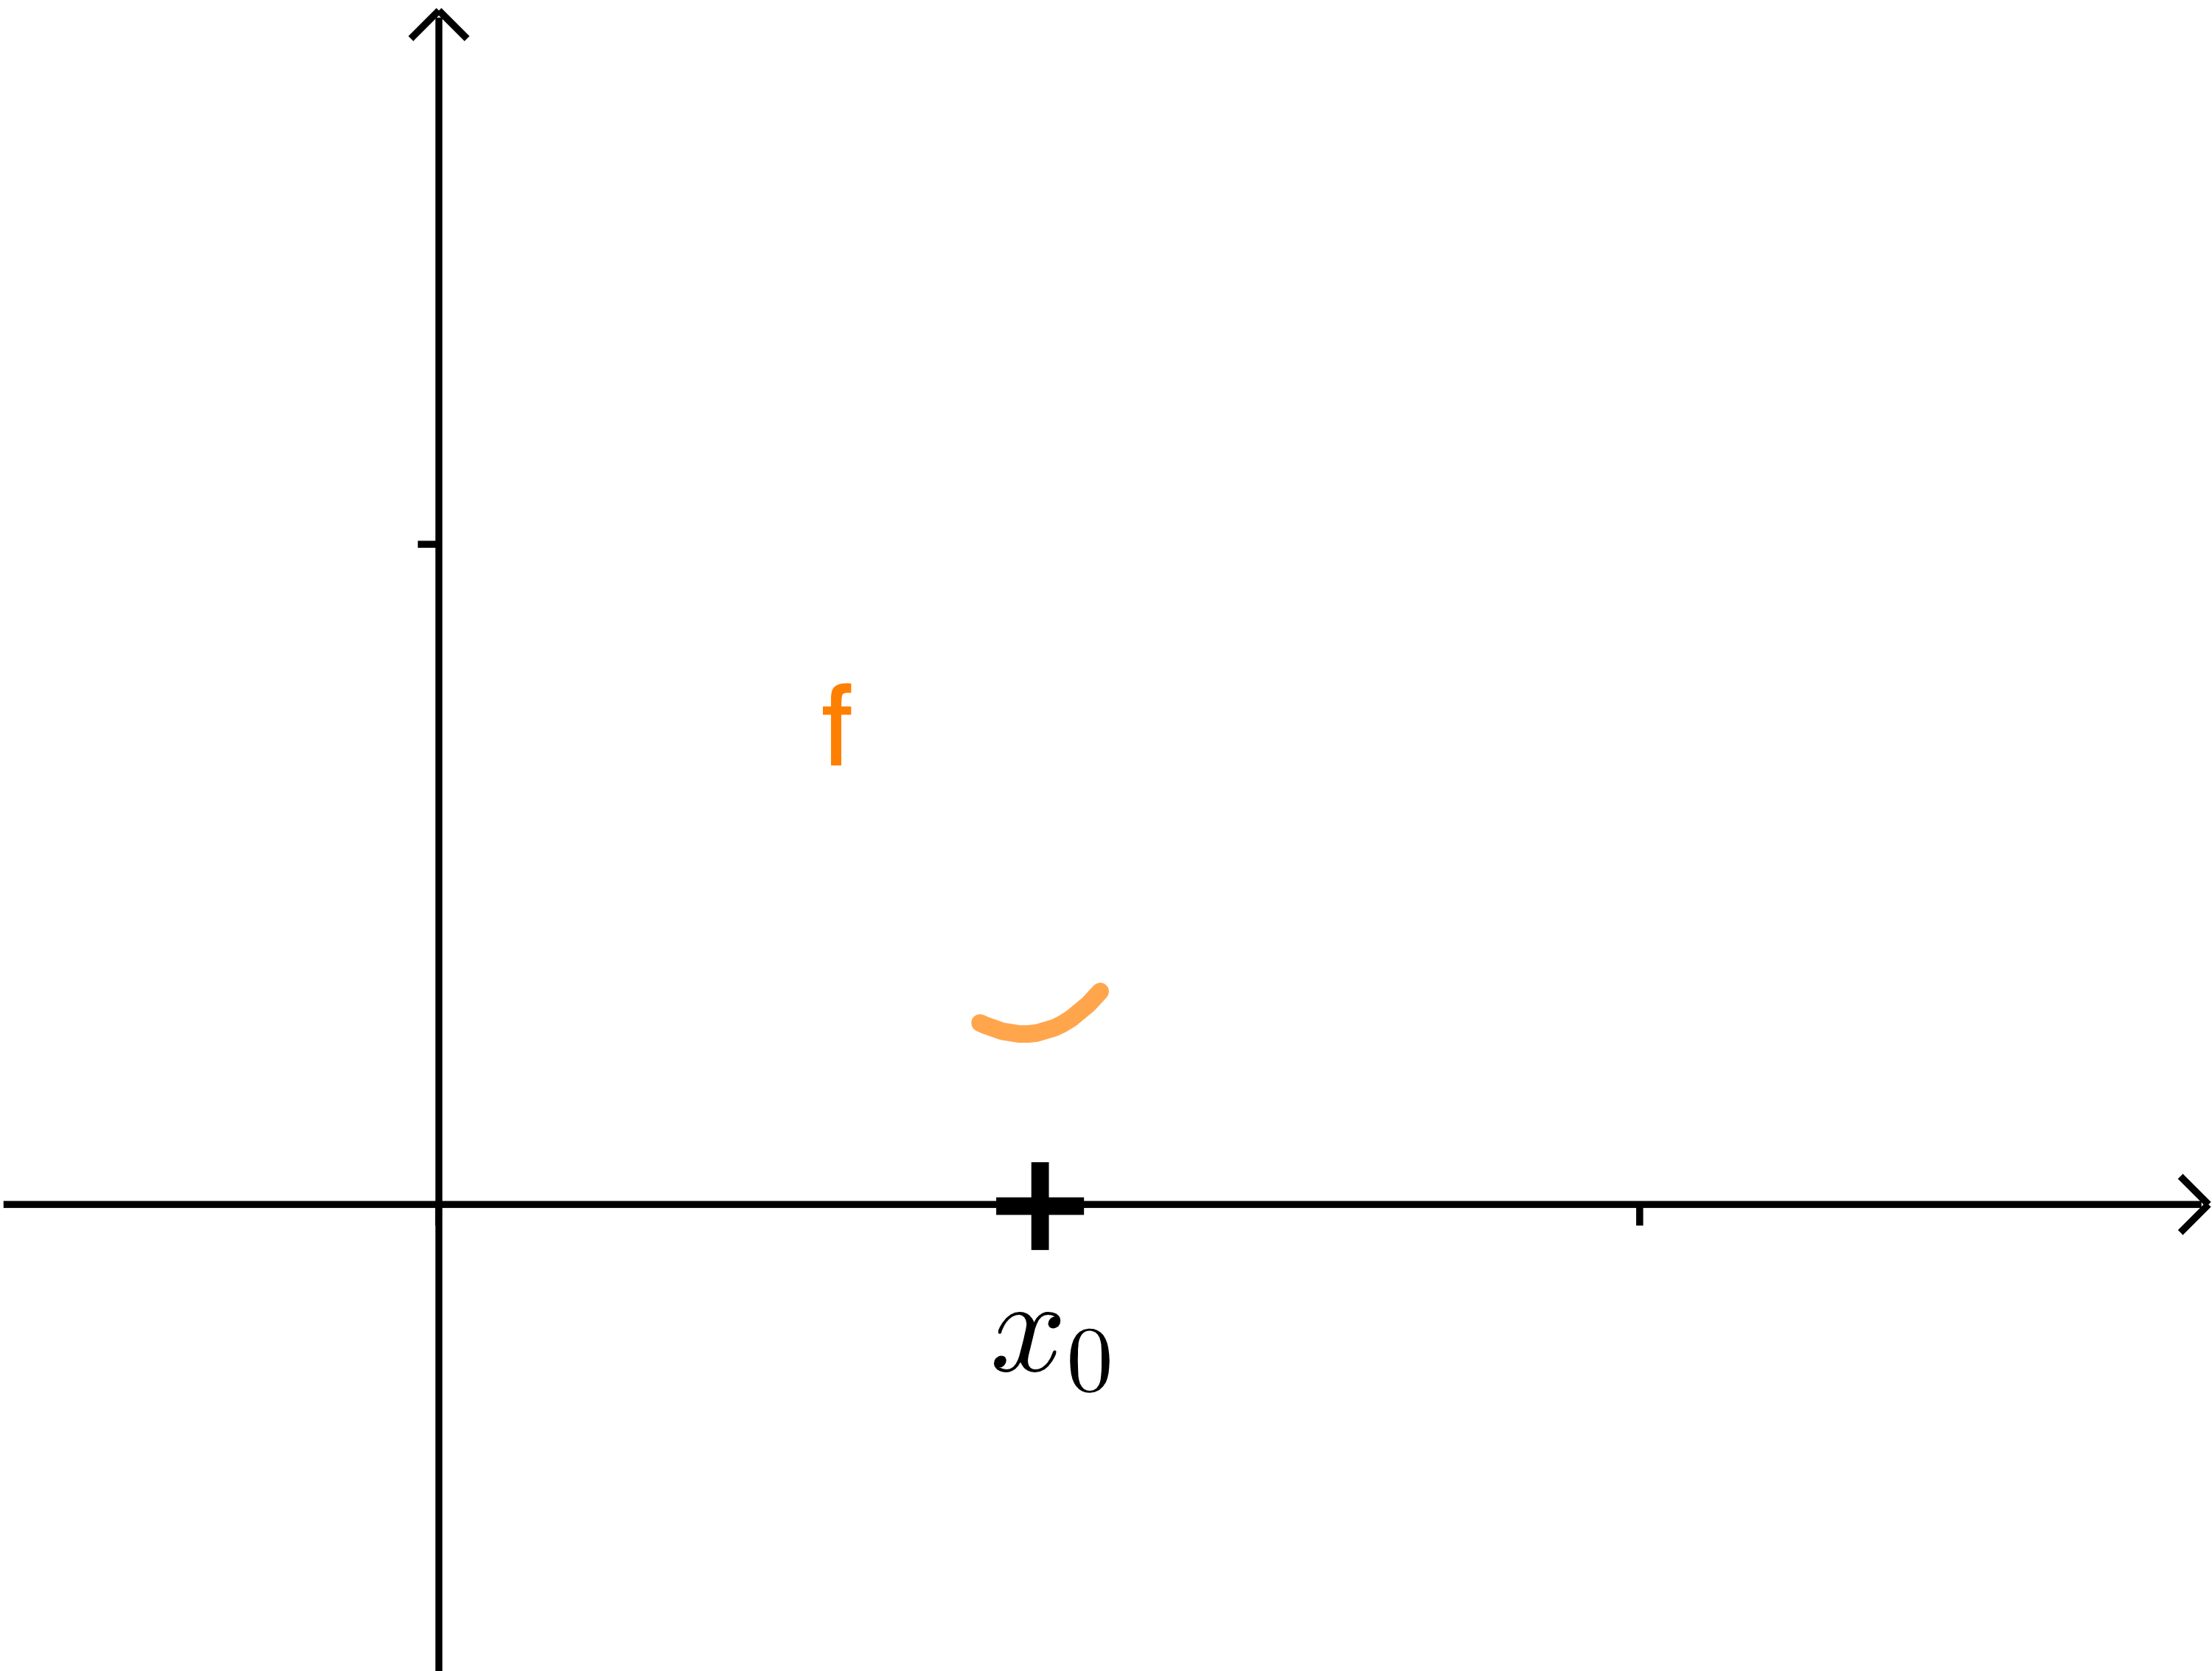
\includegraphics[width = 4cm]{media/Graph und Ableitung Kopie/min.png}\\ \hline
    \end{tabular}
\end{center}

Der Nachweis, dass eine Ableitungsfunktion $f'$ das Vorzeichen an einer bestimmen Stelle von $+$ nach $-$ oder umgekehrt wechselt, kann in der Praxis kompliziert sein. Häufiger ist es einfacher, wenn man dazu die Ableitungsfunktion $f'$ nochmals ableitet!

% \begin{definition}
%     {Höhere Ableitung}{}
%     Sei $f'$ die Ableitung einer Funktion $f$. Wenn $f'$ selbst wieder differenzierbar ist, bezeichnet man die Ableitung von $f'$ mit $f''$ und man nennt sie die zweite Ableitung von $f$.

%     Von der Funktion $f''$ lässt sich die sogenannte dritte Ableitung $f'''$ bilden u.s.w.

%     Die $n$-te Ableitung bezeichnet man mit $f^{(n)}$.

%     Einealternative Notation für die zweite, dritte und $n$-te Ableitung ist: $\frac{d^2}{dx^2}, \frac{d^3f}{dx^3}, \frac{d^nx}{dx^n}$
% \end{definition}

% \begin{bsp}
%     {Ableitungen von $f(x) = 3x^4+2x-1$}{}
%     $ f'(x) = 12x^3+2 \Rightarrow f''(x) = 36x^2 \Rightarrow f'''(x) = 72x \Rightarrow f^{(4)}(x) = 72 \Rightarrow f^{(5)}(x) = 0 \Rightarrow f^{(6)}(x) = 0, \dots$
% \end{bsp}







Wie kann man nun mit den höheren Ableitungen entscheiden, ob $f'$ an einer bestimmten Stelle das Vorzeichen von $+$ nach $-$ oder umgekehrt wechselt? Betrachten Sie dazu das folgende Beispiel:
\clearpage

\begin{bsp}
    {Von der Ableitung zum Funktionsgraphen (wird im Unterricht ergänzt)}{}
    Wie sieht der Graph einer Funktion $f$ in der Umgebung von $x=1$ aus, wenn $f(1)=4,f' (1)=0$ und $f'' (1)=2$ ist?

    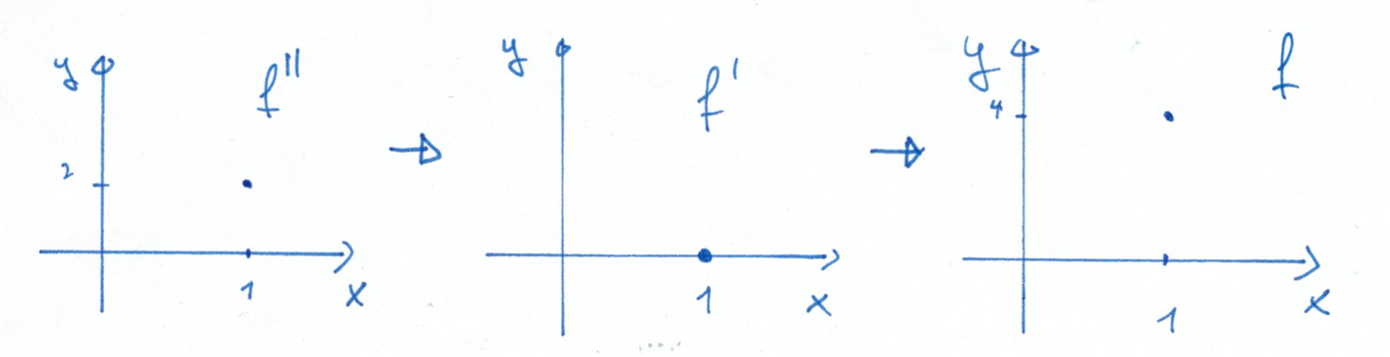
\includegraphics[width = \textwidth]{media/bspAbleitungZuGraph.png}
\end{bsp}

Merke:
\begin{definition}
    {Krümmung des Graphen}{}
    \begin{center}
    \begin{tabular}{| m{10cm} | m{4cm}|} \hline
        $f$ ist im Intervall $I$ \emph{linksgekrümmt (oder konvex)} $$\iff$$ $ f''(x) > 0$ für alle $x\in I$ & \includegraphics[width = 4cm]{media/linksgekrümmt.png}\\ \hline
        $f$ ist im Intervall $I$ \emph{rechtsgekrümmt (oder konkav)} $$\iff$$  $f''(x) < 0$ für alle $x\in I$ &\includegraphics[width = 4cm]{media/rechstgekrümmt.png}\\ \hline
        $f$ hat an der Stelle $x_0$ einen \emph{Wendepunkt} $$\iff$$ $f''$ wechselt an der Stelle $x_0$ das Vorzeichen . & 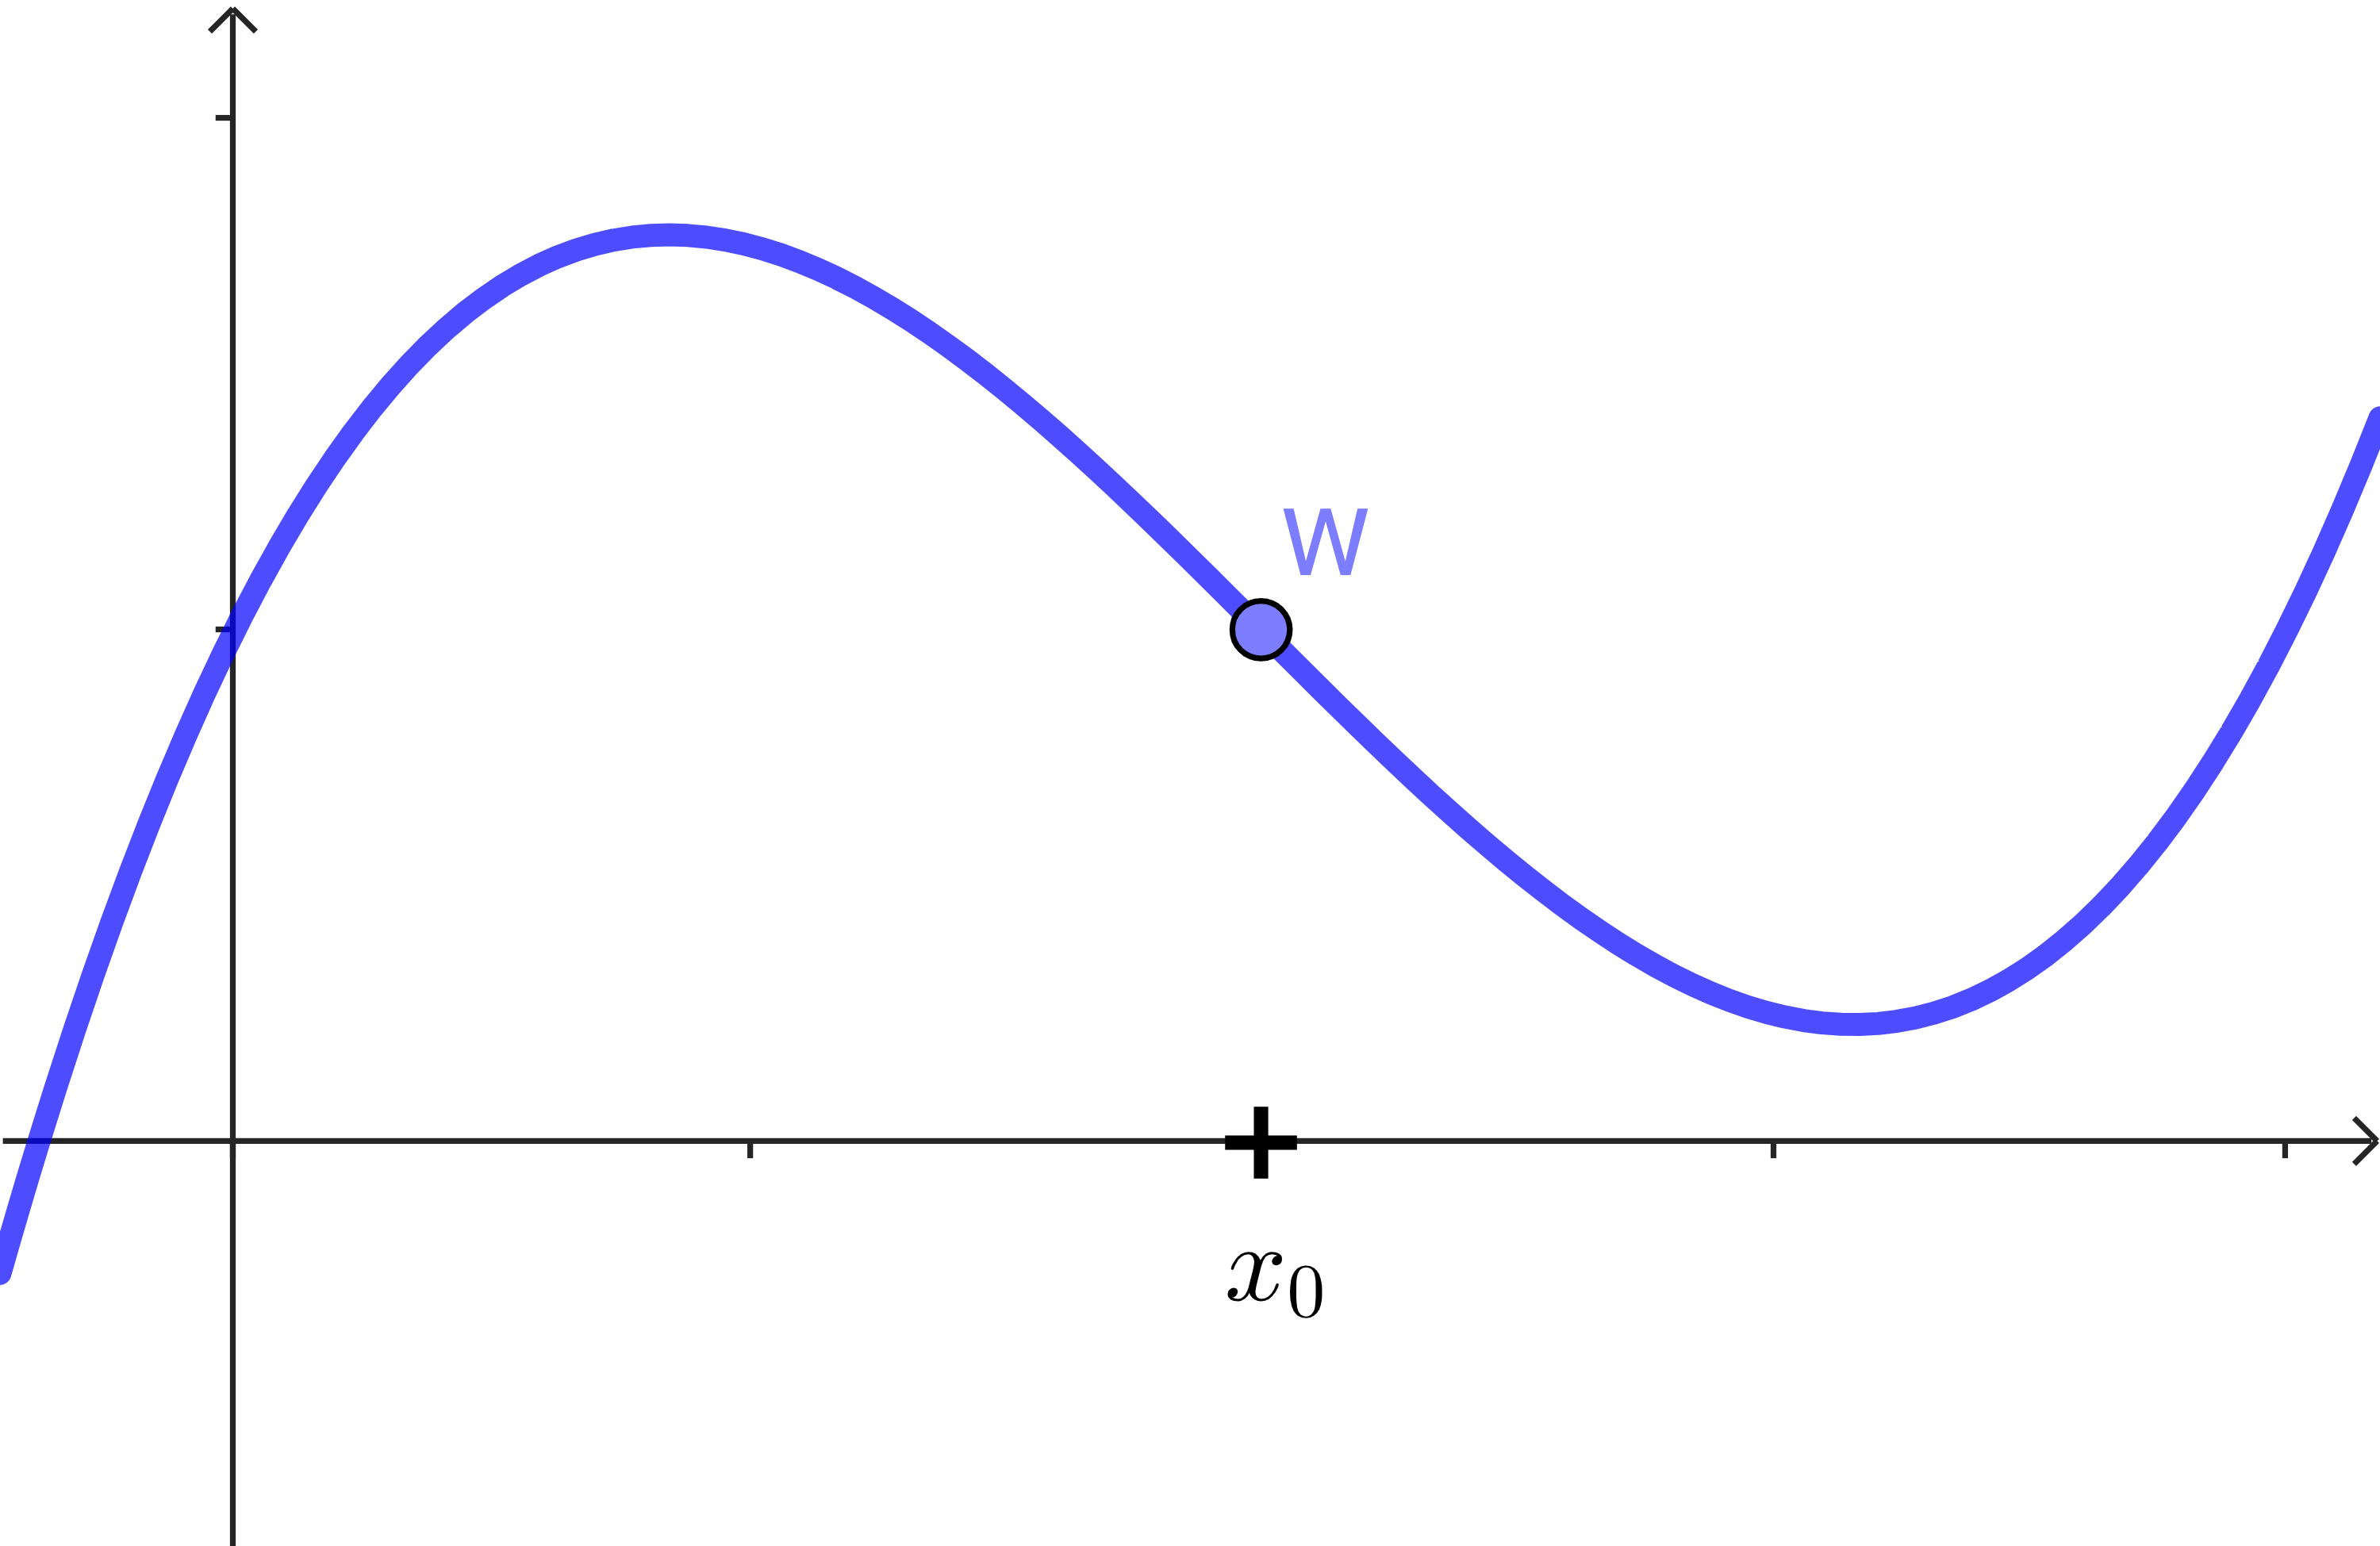
\includegraphics[width = 4cm]{media/wendept-def.png} \\ \hline
        
    \end{tabular}
\end{center}
\end{definition}

\clearpage

\begin{LA}
    {Von der Ableitung zum Funktionsgraphen}{}   
    Versuchen Sie selbst, die Informationen von links nach rechts zu übertragen, und skizzieren Sie den Graphen in einer Umgebung der markierten Punkte (mit Ausnahme der Graphen ganz links)

    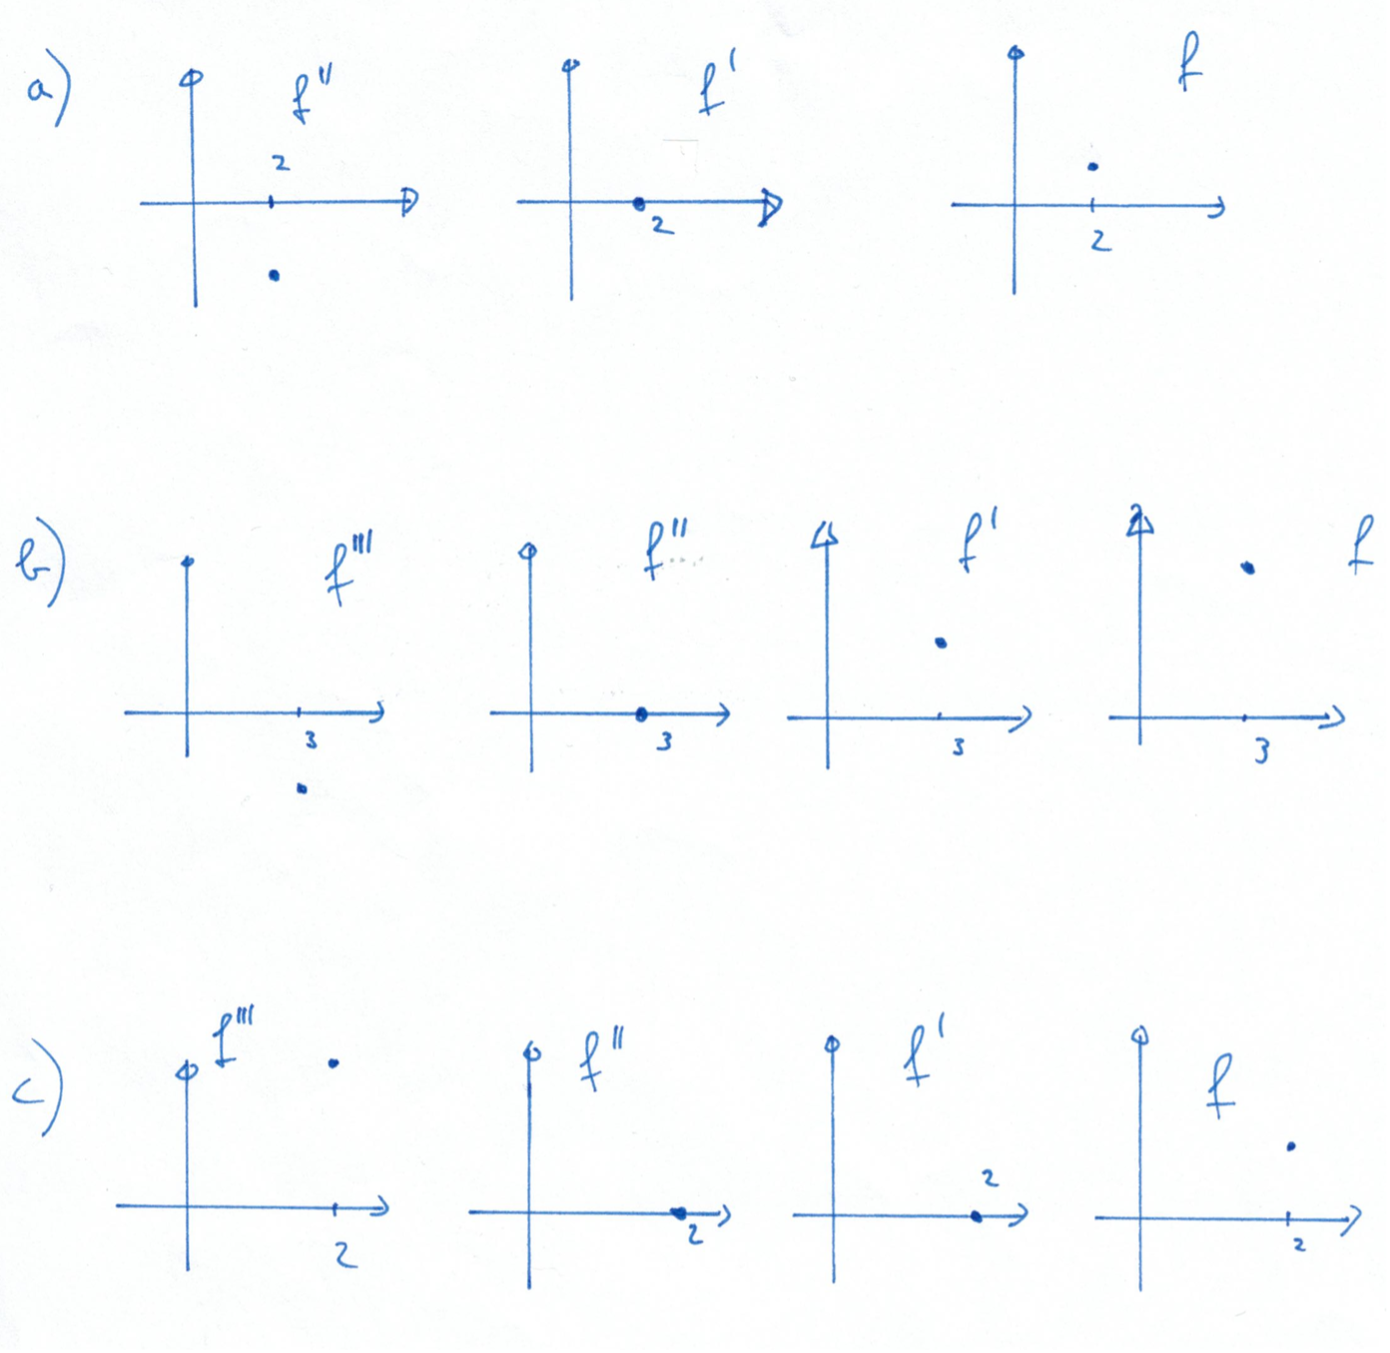
\includegraphics[width = \textwidth]{media/lavonGraphzurFu.png}
\end{LA}

\clearpage

Zusammenfassung: Hinreichende Bedingungen für spezielle Graphenpunkte

\begin{center}
    \begin{tabular}{| m{5cm} | m{5cm} | m{4cm}|} \hline
        \textbf{Hinreichende Bedingung} & \textbf{Art des Punktes} & \textbf{Bild} \\ \hline
        $$f'(x_0) = 0,$$ $$f''(x_0) < 0$$ & Lokales Maximum / Hochpunkt an der Stelle $x_0$ & 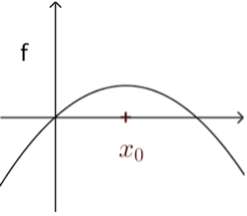
\includegraphics[width = 3.9cm]{media/lokMax.png}\\ \hline
        $$f'(x_0) = 0,$$  $$f''(x_0) > 0$$ & Lokales Minimum / Tiefpunkt an der Stelle $x_0$ & 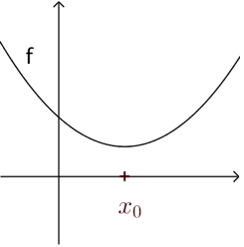
\includegraphics[width = 3.9cm]{media/lokMin.png}\\ \hline
        $$f''(x_0) = 0,$$  $$f'''(x_0) \neq 0$$ & Wendepunkt an der Stelle $x_0$ &  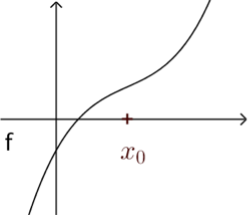
\includegraphics[width = 3.9cm]{media/wendept.png} \\ \hline
        $$f'(x_0) = 0,$$  $$f''(x_0) = 0,$$  $$f'''(x_0) \neq 0 $$ & Sattelpunkt / Terrassenpunkt an der Stelle $x_0$  \linebreak (= Wendepunkt mit horizontaler Tangente) & 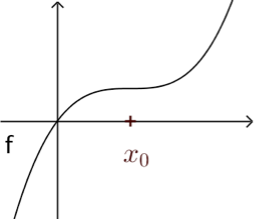
\includegraphics[width = 3.9cm]{media/sattelpt.png} \\ \hline
    \end{tabular}
\end{center}

Die speziellen Graphenpunkte haben je nach Kontext wichtige Bedeutungen. So sind z.B. Hochpunkte von Gewinnfunktionen besonders interessant, da sie den maximalen Gewinn angeben. Wendepunkte sind in der Physik oft mit einem Richtungswechsel einer Bewegung verbunden. Einige dieser Anwendungen werden wir später genauer untersuchen. Für den Moment wollen wir uns auf die mathematische Bestimmung dieser Punkte konzentrieren.
\clearpage
\begin{bsp}
{}{}
Hat die Funktion $f(x) = \frac{8}{x} -\frac{16}{x^2}$ einen Hoch- oder Tiefpunkt?

\vspace*{20 cm}
\end{bsp} 


\clearpage
Was bedeutet \emph{hinreichend}? Am Beispiel des lokalen Maximums bedeutet es das Folgende: Wenn $f'(x_0)=0$ und $f'' (x_0 )<0$ dann hat die Funktion an der Stelle $x_0$ mit Sicherheit ein lokales Maximum. \textbf{Umgekehrt aber nicht}: Wenn die Funktion an der Stelle $x_0$ ein lokales Maximum hat, dann folgt nicht unbedingt, dass die zweite Ableitung negativ ist: $f''(x_0)$ könnte auch $0$ sein.
%  Es gilt
%     $$f'(x_0) = 0, f''(x_0) > 0 \quad \Longrightarrow \text{ Tiefpunkt bei } x_0$$
%     aber
%     $$\text{ Tiefpunkt bei } x_0 \quad \cancel\Longrightarrow  \quad f'(x_0) = 0, f''(x_0) > 0 $$

\begin{bsp}
    {Hinreichende vs. notwendige Bedingungen}{hinreichendNotwendig}
    Untersuche die Funktion $f(x) = x^4-1$

    \vspace*{18cm}

\end{bsp} 

\clearpage

\begin{ueb}
    {}{}
    \begin{enumerate}
        \item Bestimme die Extrema (= Hoch- und Tiefpunkte) der Funktion  $$ f(x) = x^3 + 6x^2 - 15x + 19$$
        \item  Gegeben ist die Funktion \( f \) mit \( f(x) = x^3 + 3x^2 - 4 \).
        \begin{enumerate}
            \item Bestimme vom Graphen der Funktion \( f \) alle Tief-, Hoch- und Wendepunkte.
            \item Gib jeweils die Intervalle an, in welchen der Graph der Funktion \( f \) monoton steigt bzw. fällt.
            \item Skizziere den Graphen \( G_f \).
        \end{enumerate}
          \item Von der Funktion \( f \) ist die Funktionsgleichung 
                \[
               f(x) = 3x^4 - 8x^3 + 6x^2
                \]
                gegeben.
                \begin{enumerate}
                    \item Berechne in den Wendepunkten der Funktion \( f \) die Geradengleichungen der Tangenten (sogenannte `Wendetangenten').
                    \item In welchem Intervall ist der Graph von \( f \) links- bzw. rechtsgekrümmt?
                \end{enumerate}
        \item Zu hinreichende und notwendige Bedingungen: Bestimme die Extrema und Wendepunkte der Kurve $y=x^6-12x^5$.
        
        \item Welche Art Punkt hat die Kurve
        $$ y= \frac{1}{5} x^5 - x^4 + 2x^3 -2 x^2 + x - 1$$
        an der Stelle $x=1$?
        \item Bestimme $k\in \R$, sodass $y=x^3+kx^2+2$ bei $x= 3$ einen Wendepunkt hat.
        \item Für welchen Wert von $a\in\R$ hat die Funktion $f(x) = x^2 + \frac{a}{x}$ an der Stelle $x=-1$ ein Extremum? \\
        Handelt es sich um einen Tief- oder um einen Hochpunkt
    \end{enumerate}
\end{ueb}

\clearpage
\emph{Lösungen:}
\begin{enumerate}
    \item $H=(-5, 119), T=(1,11)$
    \item \begin{enumerate}
        \item $H=(-2, 0), T=(0, -4), W=(-1, -2)$
        \item Fallend: $]-2, 0[$, steigend $\R \setminus ]-2, 0[$
        \item \dots
    \end{enumerate}
    \item \begin{enumerate}
            \item $t_1: y= \frac{16}{9}x -\frac{5}{27}, \quad t_2: y=1$
            \item Rechtsgekrümmt: $]\frac{1}{3}, 1[$ linksgekrümmt $\R \setminus ]\frac{1}{3}, 1[$
            \end{enumerate}
    
    \item $T=(10, -200000), S =(0,0), W=(8, -131072)$
        \item Einen Sattelpunkt.
    \item $k= -9$
    \item $a=-2$, Tiefpunkt.

\end{enumerate}
































\clearpage
\subsubsection{Kurvendiskussion}
Das Ziel einer sogenannten `Kurvendiskussion' ist es, den Graphen einer Funktion möglichst genau zu beschreiben. Dazu werden in der Regel die folgenden Eigenschaften des Graphen/der Funktion bestimmt:
\begin{enumerate}
    \item Definitionsbereich und allfällige Symmetrie zum Ursprung oder zur $y$-Achse.
    \item Achsenschnittpunkte.
    \item Ableitungen.
    \item Extrema, Wende- und Sattelpunkte.
    \item Asymptotisches Verhalten für $x\to\pm\infty$ und an den Definitionslücken.
    \item Skizze des Graphs.
\end{enumerate}

\begin{bsp}
    {Diskussion der Funktion $f(x) = \frac{8x-16}{x^2}$}{}

    \phantom{Textfüler}

    \vspace*{12 cm}

    \pagebreak

    \phantom{Textfüller}

    \vspace*{21cm}

    \pagebreak

    \phantom{Textfüller}

    \vspace*{21cm}

\end{bsp}

\clearpage
\begin{ueb}
    {}{}
    \begin{enumerate}
        \item 
    Führen Sie eine Kurvendiskussion für die folgenden Polynomfunktionen durch
    \begin{enumerate}
        \item $f(x) = \frac{1}{3}\left(4x^3-x^4\right)$
        \item $g(x) = \frac{1}{3}\left(x^4-8x^3+18x^2\right)$
        \item $h(x) = \frac{1}{25}\left(x^4-32x^2+31\right)$
    \end{enumerate}
    \item Anspruchsvolle Aufgabe: Führen Sie eine Kurvendiskussion für die folgenden nicht-polynomialen Funktionen durch
    \begin{enumerate}
        \item $a(x) = \left(\frac{x-1}{x+1}\right)^2$
        \item $b(x) = \frac{1}{x} - \frac{1}{\sqrt x}$
        \item $c(x) = \sin(x) + 2\cos(x) $
        \item $d(x) = e^x (x-1)^2$
        \item $f(x) = x\ln(x)$
    \end{enumerate}
    \end{enumerate}
\end{ueb}

\clearpage
\emph{Lösungen:}

\begin{enumerate}
    \item 
    Führen Sie eine Kurvendiskussion für die folgenden Polynomfunktionen durch
    \begin{enumerate}
        \item $f(x) = \frac{1}{3}(4x^3 - x^4)$
        \begin{itemize}
            \item $D_f = \mathbb{R}$, keine Symmetrie
            \item $Y = (0, 0)$, Nullstellen: $N_1 = (0, 0)$, $N_2 = (4, 0)$
            \item $f'(x) =\frac{1}{3}(12x^2 - 4x^3) , f''(x)=\frac{1}{3}(24x - 12x^2)$ \dots
            \item Extrema: $H = (3, 9)$ \\
                  Wendepunkte: $W = (2, \frac{16}{3})$
                  Sattelpunkt $S = (0, 0)$
            \item $\lim\limits_{x \to \pm\infty} f(x) = -\infty$
        \end{itemize}

        \item $g(x) = \frac{1}{3}(x^4 - 8x^3 + 18x^2)$
        \begin{itemize}
            \item $D_g = \mathbb{R}$, keine Symmetrie
            \item $Y = (0, 0)$, Nullstellen: $N = (0,0)$
            \item $g'(x)= \frac{1}{3}(4x^3 - 24x^2 + 36x), g''(x)= \frac{1}{3}(12x^2 - 48x + 36)$ \dots
            \item Extrema: $T=(0, 0)$ \\
                  Wendepunkte: $W_1 = (1, \frac{11}{3})$
                  Sattelpunkt $S = (3, 9)$
            \item $\lim\limits_{x \to \pm\infty} g(x) = \infty$
        \end{itemize}

        \item $h(x) = \frac{1}{25}(x^4 - 32x^2 + 31)$
        \begin{itemize}
            \item $D_h = \mathbb{R}$ , $f(-x) = f(x)$ symmetrisch zur $y$-Achse.
            \item $Y = (0, 1.24)$, Nullstellen: $N = \{-5.57, -1, 1, 5.57\}$
            \item $h'(x) = \frac{1}{25}(4x^3 - 64x), h''(x)= \frac{1}{25}(12x^2 - 64)$ 
            \item Extrema: $T_1 = (-4, -9)$, $H_1 = (0, 1.24)$, $T_2 = (4, -9)$ \\
                  Wendepunkte: $W_1 = (-2.31, -4.45)$, $W_2 = (2.31, -4.45)$
            \item $\lim\limits_{x \to \pm\infty} h(x) = \infty$
        \end{itemize}
    \end{enumerate}


    \item Transzendente Funktionen
    \begin{enumerate}
        \item \( a(x) = \left( \frac{x - 1}{x + 1} \right)^2 \): 
            \begin{itemize}
            \item $D_a = \mathbb{R} \setminus \{1\}$ , keine Symmetrie
            \item $Y = (0, 1)$, Nullstellen: $N = (1,0)$
            \item $a'(x) = 4 \frac{x-1}{(x+1)^3}, a''(x) =  8 \frac{2-x}{(x+1)^4}$
            \item Extrema: $T=(1, 0)$ \\
                  Wendepunkte: $W = (2, \frac{1}{9})$
            \item $\lim\limits_{x \to \pm\infty} a(x) = 1$ \\
                $\lim\limits_{x \nearrow -1} a(x) = \lim\limits_{x \searrow -1} a(x)=\infty $
        \end{itemize}
        \item \( b(x) = \frac{1}{x} - \frac{1}{\sqrt{x}} \):
             \begin{itemize}
            \item $D_b = \mathbb{R}^+ $ , keine Symmetrie
            \item Nullstelle: $N = (1,0)$
            \item $b'(x) = \frac{\sqrt{x}-2}{2x^2}, b''(x) =  \frac{-3\sqrt{x}+8}{4x^3}$
            \item Extrema: $T=(4, -\frac{1}{4})$ \\
                  Wendepunkte: $W = (\frac{64}{9}, -\frac{15}{64})$
            \item $\lim\limits_{x \to \infty} b(x) = 0$ \\
                $\lim\limits_{x \searrow 0} b(x)=\infty $
        \end{itemize}
        \item \( c(x) = \sin(x) + 2\cos(x) \): 
            \begin{itemize}
            \item $D_c = \mathbb{R}$ , keine (einfache( Symmetrie
            \item $Y = (0, 2)$, Nullstellen: $N = (2.03 +k\cdot \pi,0), k\in \Z$
            \item $c'(x) = \cos(x) - 2 \sin(x), c''(x) =  -\sin(x)-2\cos(x)$
            \item Extrema: $T=(3.61+2k\pi, -2.24), H=(0.46+2k\pi, 2.24)$ \\
                  Wendepunkte: $W = (2.03 + k\pi, 0)$
            \item $\lim\limits_{x \to \pm\infty} c(x) $ existiert nicht.
        \end{itemize}
        \item \( d(x) = e^x(x - 1)^2 \):
            \begin{itemize}
            \item $D_d = \mathbb{R}$ , keine Symmetrie
            \item $Y = (0, 1)$, Nullstellen: $N = (1,0)$
            \item $d'(x) = e^x(x^2-1), d''(x) = e^x (x^2+2x-1)$
            \item Extrema: $T=(1,0), H=(-1, \frac{4}{e})$ \\
                  Wendepunkte: $W_1 = (-\sqrt{2}-1, 1.04), W_2 =(\sqrt{2}-1, 0.52)$
            \item $\lim\limits_{x \to \infty} d(x) = \infty, \lim\limits_{x \to -\infty} d(x) = 0$
            \end{itemize}
        \item \( f(x) = x\ln(x) \): 
            \begin{itemize}
            \item $D_f = \mathbb{R^+}$, keine Symmetrie
            \item Nullstellen: $N = (1,0)$
            \item $f'(x) = \ln(x) + 1, f''(x) = \frac{1}{x}$
            \item Extrema: $T=\left(\frac{1}{e}, -\frac{1}{e}\right)$ 
            \item $\lim\limits_{x \to \infty} f(x) = \infty$ \\
            $\lim\limits_{x \searrow 0} f(x) = 0$ (Für die Berechnung dieses Grenzwertes benötigt man spezielle Techniken (siehe Schwerpunkt :))
            \end{itemize}
    \end{enumerate}
\end{enumerate}

\clearpage
\begin{ueb}
    {Vermischte Aufgaben für \Cref{Winkel} und \Cref{speziellePte}}{}
    \begin{enumerate}
        \item Bestimme die Gleichung von Tangente und Normale im Kurvenpunkt $P$
        \begin{enumerate}
            \item $f(x) = 2x^2-5, P=(2, ?)$
            \item $g(x) = \frac{x^2+1}{x+1}, P=(-3,?)$
            \item $h(x) = \sqrt{x}, P=(4,?)$
        \end{enumerate}
           \item Berechne den Schnittwinkel der beiden Funktionsgraphen:
    \begin{enumerate}
        \item $f(x) = \frac{1}{2}x^2, \quad g(x) = \frac{1}{2}x^2-2x+6$
        \item $f(x) = \frac{2}{x^3}, \quad g(x) = 2x^3$
        \item $f(x) = e^{2x}-1, \quad g(x) = 0$
        \end{enumerate}
    \item In welchen Punkten verläuft die Kurventangente des Graphen von $f(x) = \frac{1}{3} x^3-x^2+x-4$ senkrecht zur Geraden $p: y=-\frac{1}{4}x+42$?
    \item Bestimme die Extrema und Wendepunkte der Funktion:
    \begin{enumerate}
        \item $f(x) = x^4-4x^3+4x^2$
        \item $g(x) = x + \frac{1}{x+1}$
    \end{enumerate}
    \item Eine Gleichung $n$-ten Grades hat höchstens $n$ Lösungen (\emph{Fundamentalsatz der Algebra}). \\
    Wie viele Extrema hat eine Polynomfunktion $n$-ten Grades höchstens? Und wie viele Wendepunkte?
    \item Führe eine Kurvendiskussion durch für
    \begin{enumerate}
        \item $f(x) = x^3-3x$
        \item $g(x) = x^3\cdot e^{-x}$
    \end{enumerate}
    \end{enumerate}
\end{ueb}

\clearpage
\emph{Lösungen:}
\begin{enumerate}
    \item \begin{enumerate}
        \item $t: y=8x-13 \quad n: y= -\frac{1}{8}x +\frac{26}{8}$
        \item $t: y=\frac{1}{2}x-\frac{7}{2} \quad n: y= -2x -11$
        \item $t: y=\frac{1}{4}x+1 \quad n: y= -4x +18$
    \end{enumerate}
    \item \begin{enumerate}
        \item $\varphi\approx 26.6^\circ$
        \item $\varphi_1=\varphi_2\approx 18.9^\circ$
        \item $\varphi\approx 63.4^\circ$
    \end{enumerate}
    \item $P_1 =\left(-1, -\frac{19}{3}\right), P_2 = (3,-1 )$
    \item \begin{enumerate}
        \item $T_1 = (0,0), W_1 \approx(0.42, 0.44) , H =(1,1), W_2\approx(1.58, 0.44), T_2=(2,0)$
        \item $T=(0, 1), H = (-2, -3)$, keine Wendepunkte. 
    \end{enumerate}
    \item Höchstens $n-1$ Extrema und $n-2$ Wendepunkte.
    \item \begin{enumerate}
                \item \begin{itemize}
                    \item $D = \mathbb{R}$ , Punktsymmetrisch zum Ursprung ($f(-x) = -f(x)$)
                    \item $Y = (0, 0)$, Nullstellen: $N_1 = (0,0), N_{2,3} = (\pm \sqrt{3}, 0)$
                    \item $f'(x) =3x^2-3, f''(x) = 6x$
                    \item Extrema: $T=(1,-2), H=(-1, 2)$ \\
                        Wendepunkte: $W = (0, 0)$
                    \item $\lim\limits_{x \to \infty} f(x) = \infty, \lim\limits_{x \to -\infty} f(x) = -\infty$
                    \end{itemize}
                \item \begin{itemize}
                    \item  $D = \mathbb{R}$ 
                    \item $Y = (0, 0)$, Nullstellen: $N = (0,0)$
                    \item $g'(x) = e^{-x} (3x^2-x^3), g''(x) = e^{-x} (x^3-6x^2+6x)$
                    \item Extrema: $ H=(3, 1.34)$ \\
                        Wendepunkte: $W_1 \approx (1.27, 0.57), W_2 \approx(4.73, 0.93)$ \\
                        Sattelpunkt $S=(0,0)$
                    \item $\lim\limits_{x \to \infty} g(x) =0, \lim\limits_{x \to -\infty} g(x) = -\infty$
                \end{itemize}
    \end{enumerate}
 
    
\end{enumerate} 